\documentclass{beamer}

\usepackage[utf8]{inputenc}
\usepackage{hyperref}

\usetheme{Berkeley}
\beamertemplatenavigationsymbolsempty
\setbeamertemplate{headline}{}
 
\title{Highlighting in FoodChain-Lab}
\date{}
 
\begin{document}
\maketitle

\section{Aufgaben}
\begin{frame}
	\begin{itemize}
		\item Nutzen Sie folgenden Workflow: \url{https://github.com/SiLeBAT/BfROpenLabResources/raw/master/GitHubPages/workflows/Small_Example.zip}.
		\item Ändern Sie im \textbf{Tracing View} die Farbe für Ausbruchs-Stationen (\textbf{Outbreak}) von rot auf türkis.
		\item Fügen Sie zu jeder Station das Label "node" hinzu.
	\end{itemize}
\end{frame}
 
\section{1}
\begin{frame}
	\begin{center}
  		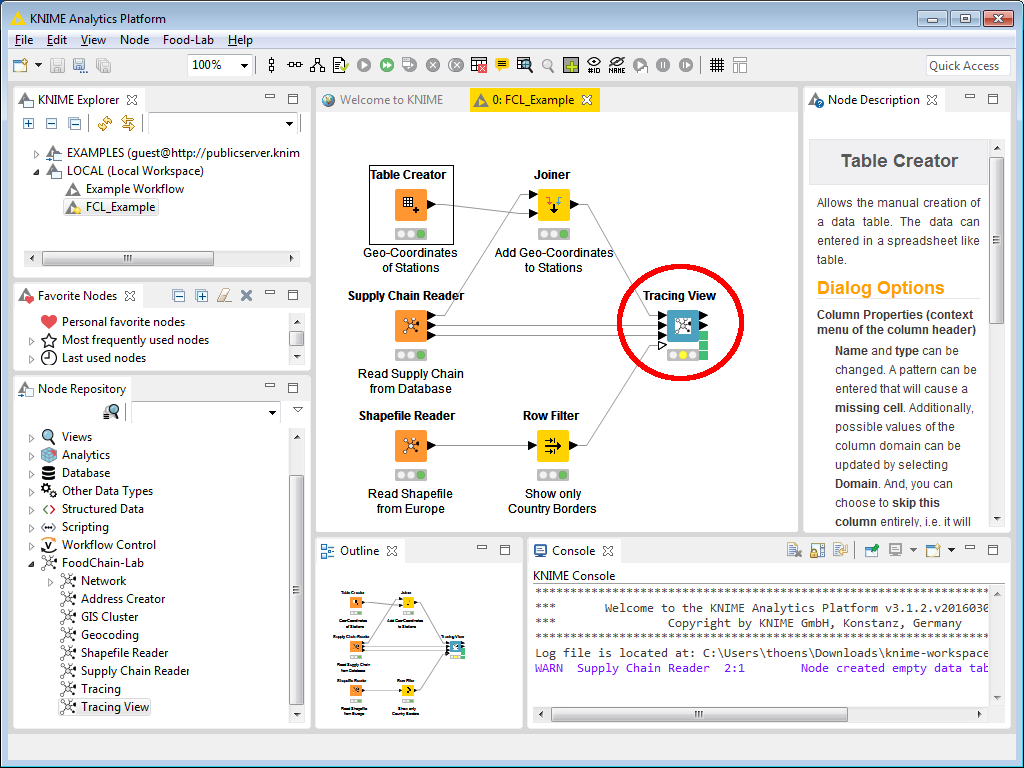
\includegraphics[height=0.6\textheight]{1.png}
	\end{center}
	\begin{itemize}
		\item Importieren Sie den Small Example Workflow von \url{https://github.com/SiLeBAT/BfROpenLabResources/raw/master/GitHubPages/workflows/Small_Example.zip}.
		\item Öffnen Sie den \textbf{Tracing View} per Doppelklick.
	\end{itemize}
\end{frame}

\section{2}
\begin{frame}
	\begin{center}
  		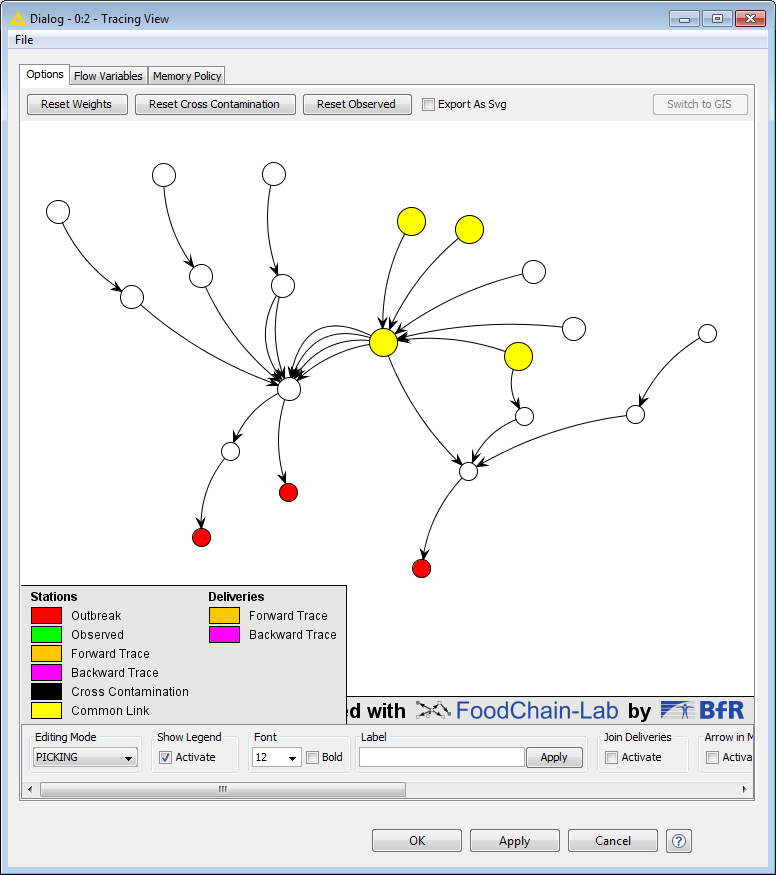
\includegraphics[height=0.6\textheight]{2.png}
	\end{center}
	\begin{itemize}
		\item Hier sehen Sie einen kleinen Liefergraphen mit drei Ausbruchs-Stationen (rot) im unteren Teil.
	\end{itemize}
\end{frame}

\section{3}
\begin{frame}
	\begin{center}
  		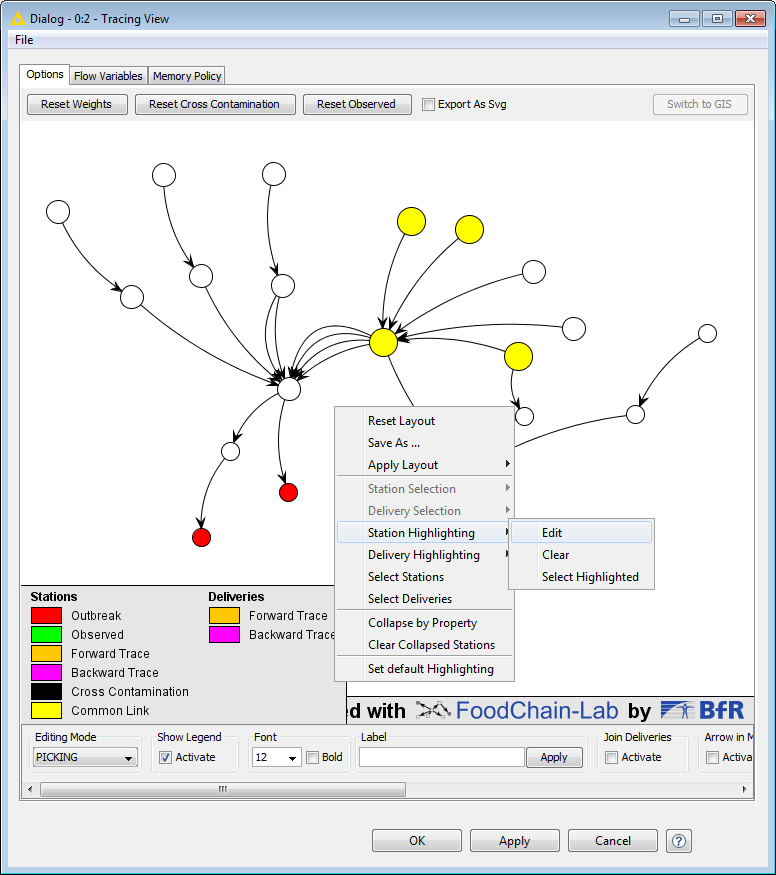
\includegraphics[height=0.6\textheight]{3.png}
	\end{center}
	\begin{itemize}
		\item Nun werden wir die Farbe der Ausbruchs-Stationen (\textbf{Outbreak}) ändern.
		\item Machen Sie einen Rechtsklick in den Graphen und wählen Sie \textbf{Station Highlighting $>$ Edit}.
	\end{itemize}
\end{frame}

\section{4}
\begin{frame}
	\begin{center}
  		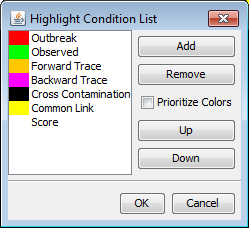
\includegraphics[height=0.6\textheight]{4.png}
	\end{center}
	\begin{itemize}
		\item Ein Dialog mit den definierten Highlighting-Bedingungen erscheint.
		\item Machen Sie einen Doppelklick auf die \textbf{Outbreak}-Bedingung um diese zu editieren.
	\end{itemize}
\end{frame}

\section{5}
\begin{frame}
	\begin{center}
  		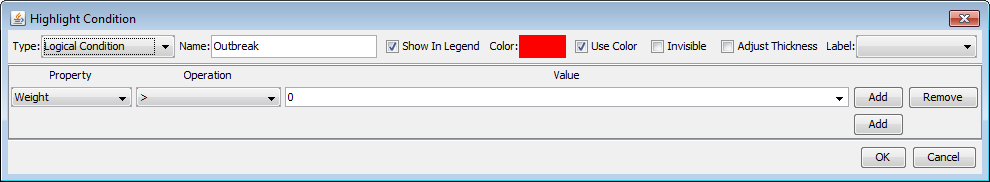
\includegraphics[width=0.9\textwidth]{5.png}
	\end{center}
	\begin{itemize}
		\item Ein neuer Dialog zum Editieren der \textbf{Outbreak}-Bedingung erscheint.
		\item In diesem Dialog können Sie definieren auf welche Stationen das Highlighting angewendet wird.
		\item Derzeit wird es auf alle Stationen mit "Weight" $>$ 0 angewendet. Sie können weitere Ausdrücke hinzufügen indem Sie rechts auf einen \textbf{Add}-Button klicken. Mehrere Ausdrücke können via "And" oder "Or" verknüpft werden.
		\item Zum Editieren der Farbe klicken Sie auf das rote Rechteck neben \textbf{Color}.
	\end{itemize}
\end{frame}

\section{6}
\begin{frame}
	\begin{center}
  		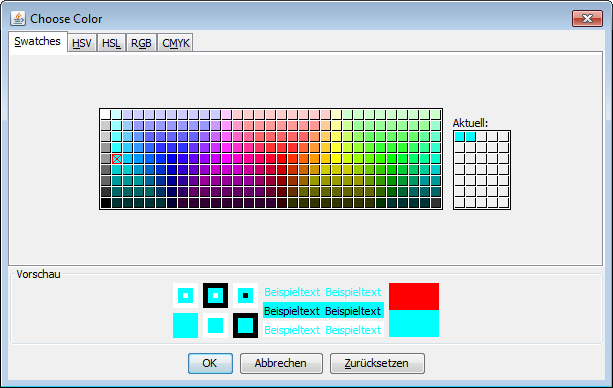
\includegraphics[height=0.6\textheight]{6.png}
	\end{center}
	\begin{itemize}
		\item In dem Farbauswahl-Dialog wählen türkis und klicken Sie \textbf{OK}.
	\end{itemize}
\end{frame}

\section{7}
\begin{frame}
	\begin{center}
  		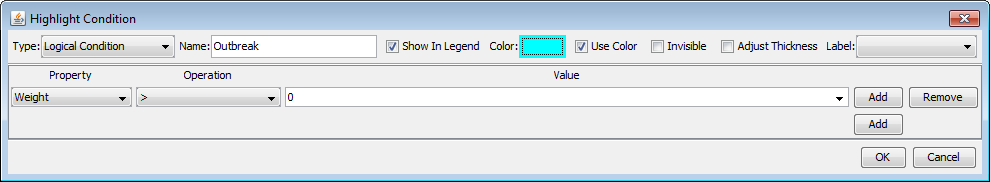
\includegraphics[width=0.9\textwidth]{7.png}
	\end{center}
	\begin{itemize}
		\item Das Rechteck neben \textbf{Color} sollte jetzt türkis sein.
		\item Klicken Sie \textbf{OK}.
	\end{itemize}
\end{frame}

\section{8}
\begin{frame}
	\begin{center}
  		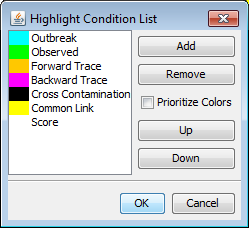
\includegraphics[height=0.6\textheight]{8.png}
	\end{center}
	\begin{itemize}
		\item In dem Dialog mit allen Highlight-Bedingungen klicken Sie \textbf{OK} um ihre Änderungen zu übernehmen.
	\end{itemize}
\end{frame}

\section{9}
\begin{frame}
	\begin{center}
  		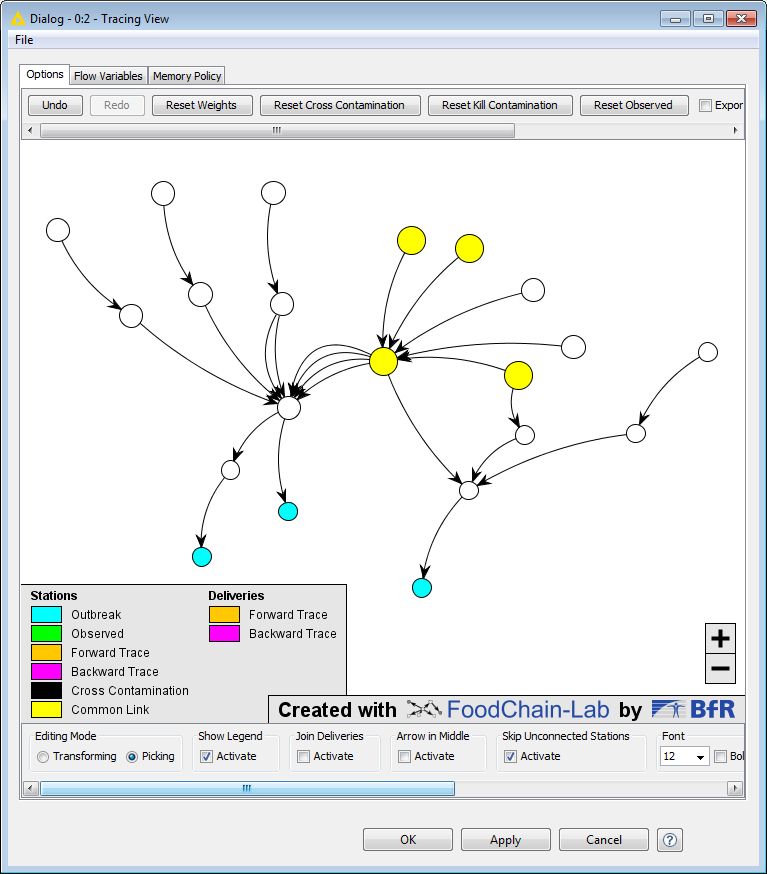
\includegraphics[height=0.6\textheight]{9.png}
	\end{center}
	\begin{itemize}
		\item Die Ausbruchs-Station im Graphen sollten jetzt türkis sein.
	\end{itemize}
\end{frame}

\section{10}
\begin{frame}
	\begin{center}
  		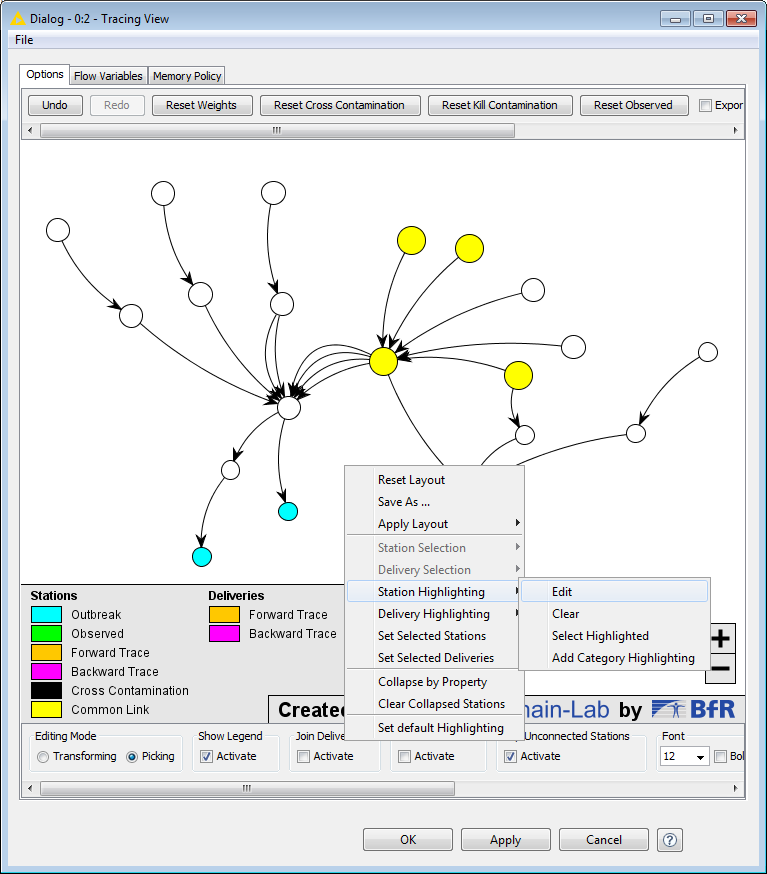
\includegraphics[height=0.6\textheight]{10.png}
	\end{center}
	\begin{itemize}
		\item Nun wollen wir allen Stationen ein Label geben.
		\item Machen Sie einen Rechtsklick in den Graphen und wählen Sie \textbf{Station Highlighting $>$ Edit}.
	\end{itemize}
\end{frame}

\section{11}
\begin{frame}
	\begin{center}
  		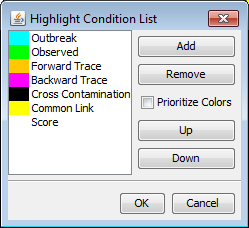
\includegraphics[height=0.6\textheight]{11.png}
	\end{center}
	\begin{itemize}
		\item Das Labeln werden wir als neue Highlight-Bedingung hinzufügen.
		\item Klicken Sie \textbf{Add} zum Erstellen einer neuen Bedingung.
	\end{itemize}
\end{frame}

\section{12}
\begin{frame}
	\begin{center}
  		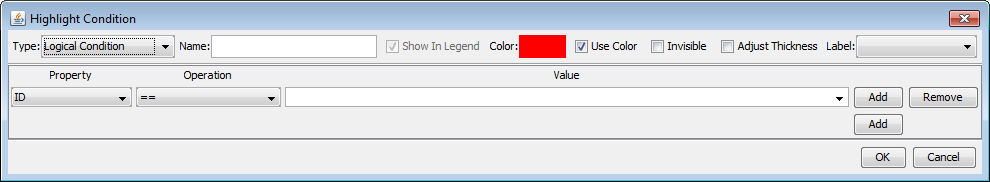
\includegraphics[width=0.9\textwidth]{12.png}
	\end{center}
	\begin{itemize}
		\item Ein Dialog erscheint, in dem Sie die gewünschte Highlight-Bedingung definieren können.
	\end{itemize}
\end{frame}

\section{13}
\begin{frame}
	\begin{center}
  		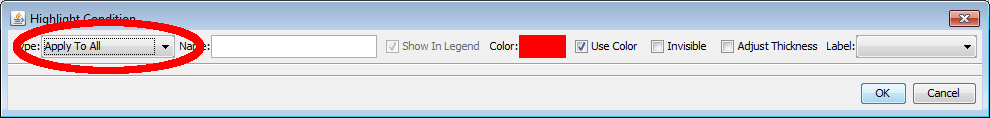
\includegraphics[width=0.9\textwidth]{13.png}
	\end{center}
	\begin{itemize}
		\item Da die Bedingung für alle Stationen gelten soll, setzen Sie den \textbf{Type} auf "Apply To All".
	\end{itemize}
\end{frame}

\section{14}
\begin{frame}
	\begin{center}
  		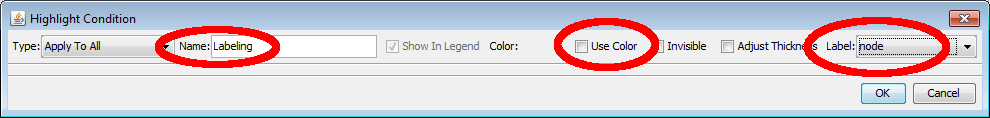
\includegraphics[width=0.9\textwidth]{14.png}
	\end{center}
	\begin{itemize}
		\item Setzen Sie \textbf{Name} auf "Labeling" (zur besseren Dokumentation).
		\item Deaktivieren Sie \textbf{Use Color}, da wir nur Label erstellen und keine Farben vergeben wollen.
		\item Setzen Sie \textbf{Label} auf "node", da dies die Spalte mit den Namen der Stationen ist.
		\item Drücken Sie \textbf{OK} um die Highlight-Bedingung zu erzeugen.
	\end{itemize}
\end{frame}

\section{15}
\begin{frame}
	\begin{center}
  		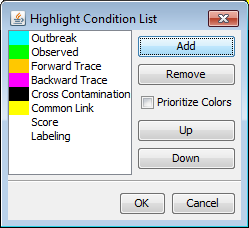
\includegraphics[height=0.6\textheight]{15.png}
	\end{center}
	\begin{itemize}
		\item In dem Dialog mit allen Highlight-Bedingungen sollten Sie nun eine neue Bedingung "Labeling" sehen.
		\item Drücken Sie \textbf{OK} um ihre Änderungen zu übernehmen.
	\end{itemize}
\end{frame}

\section{16}
\begin{frame}
	\begin{center}
  		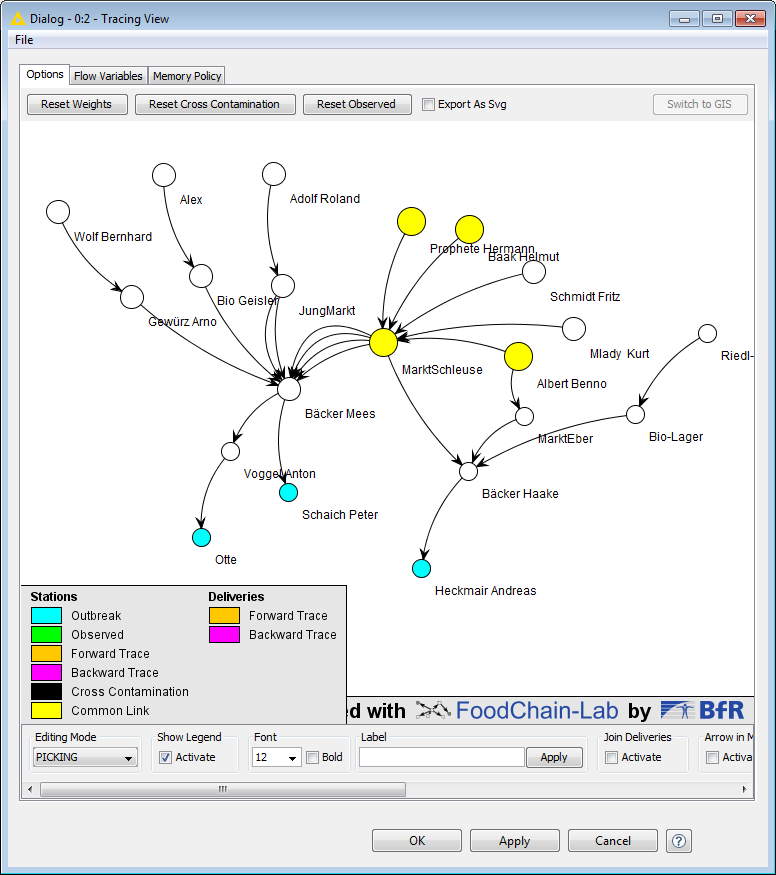
\includegraphics[height=0.6\textheight]{16.png}
	\end{center}
	\begin{itemize}
		\item Im Graphen sollten Sie nun ein Label neben jeder Station sehen.
	\end{itemize}
\end{frame}

\section{17}
\begin{frame}
	\begin{center}
  		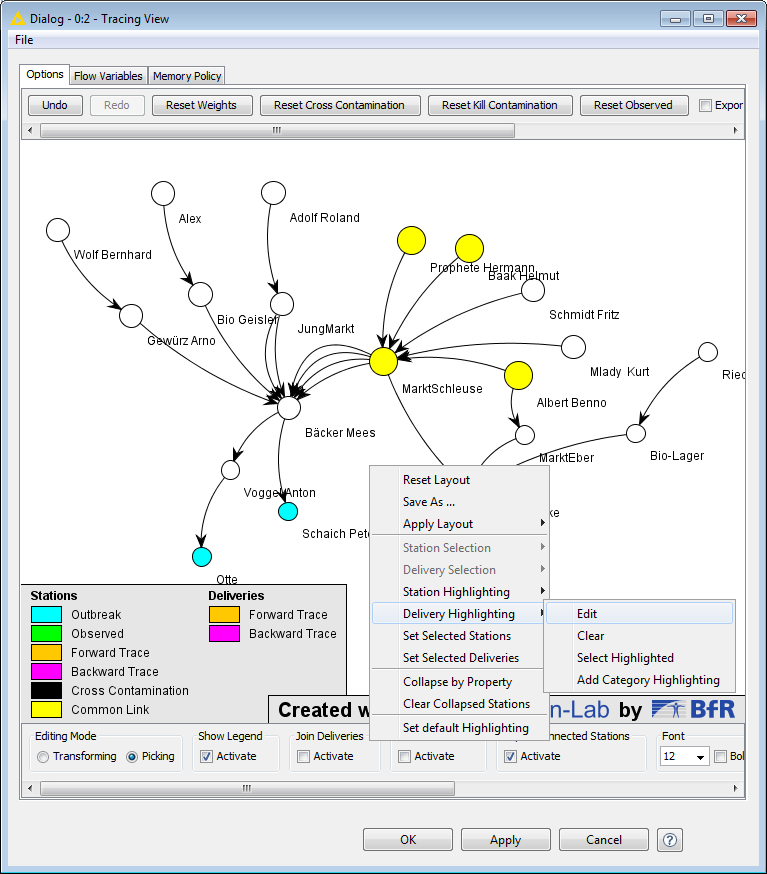
\includegraphics[height=0.55\textheight]{17.png}
	\end{center}
	\begin{itemize}
		\item Lieferungen können auf dieselbe Art und Weise gefärbt und gelabelt werden, wie wir es gerade für Stationen gemacht haben.
		\item Um den Dialog zum Editieren der Highlight-Bedingungen für Lieferungen zu öffnen, machen Sie einen Rechtsklick in den Graphen und wählen Sie \textbf{Delivery Highlighting $>$ Edit}.
	\end{itemize}
\end{frame}

\end{document}